\documentclass[12pt, a4paper, final]{report}

%Encoding
%--------------------------------------
\usepackage[utf8]{inputenc}
\usepackage[T1]{fontenc}
%--------------------------------------

%French-specific commands
%--------------------------------------
%\usepackage[frenchb]{babel}
\usepackage[autolanguage]{numprint}
%--------------------------------------

%Hyphenation rules
%--------------------------------------
%\usepackage{hyphenat}
%\hyphenation{mathéma-tiques récu-pérer}
%--------------------------------------

% Liens hypertext
%--------------------------------------
\usepackage{hyperref}

% Folder tree
%--------------------------------------
\usepackage{dirtree}

%Other package
%--------------------------------------
\usepackage{titlesec} %titleformat
\usepackage{graphicx} %graphics
\usepackage{caption}
\usepackage{subcaption}
%--------------------------------------

%Disable "Chapter" before your chapter section
\titleformat{\chapter}[hang]{\bf\huge}{\thechapter}{2pc}{}

%%%%%%%%%%%%%%%%%%%%%%%%%%%%%%%%%%%%%%%%%%%%%

% Glossary
\usepackage[acronym]{glossaries}
\makeglossaries
\newglossaryentry{App}
{
    name={\textsc{App}}, 
    description={Application}
}

%%%%%%%%%%%%%%%%%%%%%%%%%%%%%%%%%%%%%%%%%%%%%

\begin{document}

%%%%%%%%%%%%%%%%%%%%%%%%%%%%%%%%%%%%%%%%%%%%%

\begin{titlepage}

    \centering
    
    \includegraphics[width=0.75\textwidth]{./img/c00-main/logo.png}
    \par\vspace{1cm}
    {\scshape Hämeen ammattikorkeakoulu \\Hämeen ammattikorkeakoulu \par}
    \vspace{1cm}
    
    {\scshape\Large Project Report\par}
    \vspace{1.5cm}
    
    {\huge\bfseries Transportation modeling and Web content\par}
    \vspace{2cm}
    
    {\Large\itshape František Kolovský and Pierre-Vincent Vrot\par}
    \vfill
    
    Erasmus Exchange from \par
    \textsc{ZCU} ... \par
    \textsc{IMERIR} Institut Méditerranéen d’Étude et de Recherche en Informatique et Robotique \par

    \vfill
    
    {\large \today  \par version 0.1 \par}
    
\end{titlepage}

% Paragraphes spaces
%\setlength{\parindent}{4em}
\setlength{\parskip}{1em}
%\renewcommand{\baselinestretch}{1.5}

%%%%%%%%%%%%%%%%%%%%%%%%%%%%%%%%%%%%%%%%%%%%%

%Empty page
%--------------------------------------
\newpage
\null
\newpage

%%%%%%%%%%%%%%%%%%%%%%%%%%%%%%%%%%%%%%%%%%%%%

% INTRODUCTION
%--------------------------------------

\chapter*{Abstract}
\addcontentsline{toc}{chapter}{Abstract}
% ABSTRACT
%%%%%%%%%%%%%%%%%%%%%%%%%%%%%%%%%%%%%%%%%%%%%

% FRENCH
%%%%%%%%%%%%%%%%%%%%%%%%%%%%%%%%%%%%%%%%%%%%%

%Les Systèmes d'Information Géographique (SIG) permettent, entre autres, d'acquérir, de traiter, d'organiser et de présenter des données géographiques, produisant ainsi des plans clairs, précis et intuitifs, et ce, à travers une composante web accessible depuis n'importe quel navigateur.

%Le projet TraMap, proposé par HAMK et supervisé par Ramboll, est un outil simple et flexible permettant à un utilisateur de consulter des informations d'habitudes de transport issues de données géographiques en open source et d'en obtenir les informations sous forme d'application web et mobile.

%C'est dans le cadre de ce besoin d'outil de consultation et d'exploitation des données que s'inscrit notre projet. Notre rôle est de rechercher des données open sources disponibles sur internet, d'en extraire les informations pour contruire un modèle d'habitude de transport, puis de développer une application de consultation des données multiplateformes. \\ \\

% KEYWORDS
%\par
%\smallskip
%\noindent \textbf{Keywords:} SIG, Modèle de Transport, Web, Algorithme, Sources Libres

% ENGLISH
%%%%%%%%%%%%%%%%%%%%%%%%%%%%%%%%%%%%%%%%%%%%%

The Geographic Information Systems (GIS) allow, among others, to acquire, to treat, to organize and to present geographical data, to produce clear, accurate and intuitive maps, via an accessible web component from any browser.

The TraMap project, proposed by HAMK and supervised by Ramboll, is a simple and flexible tool that allows a user to view the transportation habits of information from open source geographic data and show informations in an application (web or mobile).

It in this context, of consultation tool and operating data, that our project takes place. Our role is to look for open data sources available on the Internet, to extract the information, to build an usual transport model and then develop a consultation multiplatform web application. \\ \\


% KEYWORDS
\par
\smallskip
\noindent \textbf{Keywords:} GIS, Transport Modeling, Web, Algorithm, Open Sources

\chapter*{Acknowledgments}
\addcontentsline{toc}{chapter}{Remerciements}
% Acknowledgments
%%%%%%%%%%%%%%%%%%%%%%%%%%%%%%%%%%%%%%%%%%%%%

% FR
Il nous est agréable de nous acquitter d’une dette de reconnaissance auprès de toutes les personnes dont l’intervention au cours de ce projet a favorisé son aboutissement ainsi que toutes les personnes ayant participé, de près ou de loin, à notre formation.

Dans un premier temps, nous tenons à présenter nos sincères remerciements à Mr. Jari Mustajärvi, responsable de la formation TIC (Technologies de l'information et de la Communication), pour son accueil chaleureux au sein de HAMK et pour nous avoir permis de vivre une expérience très enrichissante.

Nos plus grands remerciements vont à Mr Janne Rautio, notre responsable de projet, pour sa disponibilité et ses encouragements tout au long de ce projet et dont les directives précieuses et les conseils pertinents nous ont été d’un appui considérable dans nos démarches ; Mme. Taina Haapämaki pour ses directives, son expertise et son implication dans notre projet.

Nous tenons également à adresser nos remerciements à nos écoles respectives, University of West Bohemia et l'IMERIR, pour nous avoir proposé cet Erasmus enrichissant, et ce, dans un cadre agréable de complicité et de respect.

Enfin, que tous ceux et celles qui ont contribué de près ou de loin à l’accomplissement de ce travail trouvent l’expression de nos remerciements les plus chaleureux.




\setlength{\parskip}{0em}
\tableofcontents
\setlength{\parskip}{1em}

% MAIN
%--------------------------------------
\chapter*{Introduction}
\addcontentsline{toc}{chapter}{Introduction}
% Introduction
%%%%%%%%%%%%%%%%%%%%%%%%%%%%%%%%%%%%%%%%%%%%%

% FRENCH
%%%%%%%%%%%%%%%%%%%%%%%%%%%%%%%%%%%%%%%%%%%%%
Dans une Finlande où le vélo, la marche à pieds et les transports en communs sont de plus en plus utilisés, il devient nécessaire de se munir de moyens d'informations les plus utiles possibles afin de pouvoir anticiper les déplacements.

A l’ère actuelle, les entreprises sont toujours à l’affût de nouveautés, notamment dans le domaine SIG, que ce soit question de nouveaux outils ou de technologie. Chaque entreprises développent et commercialisent leurs outils d'information traffic. C'est dans une optique de partage de l'information, et du libre accès que va s'axer notre projet.

Aujourd'hui, open source et open data sont des sources d'information de plus en plus utilisées et permettent d'évoluer en communauté coopérative. Notre objectif principal, pour la réalisation de ce projet, est de récupérer les données et les outils open sources sur lesquels n'importe qui pourrait s'appuyer pour développer un modèle de consultation de données sur les habitudes de transport d'une ville. Notre cadre de recherche s'axera sur la ville de Hyvinkää et des données de déplacement à vélo.

Le travail réalisé se découpe en trois grandes parties : la première consiste à déterminer le modèle de transport théorique et mathématique des données qui seront consommées ; la seconde explique la façon dont une application peut être développée pour la consultation des données ; et enfin la troisième, et dernière partie, permet de combiner les précédentes parties afin d'obtenir un résultat consultable sur différentes plateformes.


\chapter{Transportation Modeling}
\section{Transportation model}
In upcoming section following expressions will be used:

\begin{tabular}{ll}
$T$ & transportation matrix (number of trips between zones)\\
$C$ & travel cost matrix (between zones) \\
$T_i, T_j$ & sum value in row/column in $T$\\
$n$ & number of zones (size of matrix)
\end{tabular}

\subsection{Trip destination}

For determine transportation matrix $T$ was used Gravity model:
$$T_{ij} = K_i K_j T_i T_j f(C_{ij})$$
where
$$T_i = \sum_{j = 1}^{n} T_{ij}$$
$$T_j = \sum_{i = 1}^{n} T_{ij}$$
$$K_i = \frac{1}{\sum_{j} K_j T_j f(C_{ij})}$$
$$K_j = \frac{1}{\sum_{i} K_i T_i f(C_{ij})}$$
where in our case $$f(x) = x^{-2}$$.
$T_i$ is number of trips outcoming from the zone (origin in the zone) $i$, $T_j$ is number of trips incoming to the zone (destination in zone) $j$. So sometimes transportation matrix is called \textit{OD Matrix}. 

Now we must determine $K_i$ and $K_j$. We used iterative proportional fitting. It is iterative solution. Fist we compute $T^1$ with $K_i, K_j = 1$. After we can use iteration equation for $T$:
$$T_{ij}^{m} = \frac{Z_i}{T_i^{m-1}} T_{ij}^{m-1}$$
$$T_{ij}^{m} = \frac{Z_j}{T_j^{m-1}} T_{ij}^{m-1}$$
where $Z_i$ and $Z_j$ are origin and destination trips (we know), $m$ is iteration.

\subsection{Count traffic}
Now we know how many people travel from zone $i$ to zone $j$, so we can find path from $i$ to $j$ and 
attributed this value into every edges in path.

In our solution we compute N paths for every pair of zones. Every path is based on another cost. Cost is based on length, time and vertical distance. Final cost is linear combination these partition cost.
$$c = \left(\begin{array}{ccc}
k_t & k_l & k_h\\
\end{array}\right) \left( \begin{array}{c}
t\\
l\\
h\\
\end{array} \right)$$

where $c$ is cost, $t$ is time, $l$ is length and $h$ is vertical distance. Number of trip is split evenly among all the paths.
\section{Implementation}
In upcoming section following expressions will be used:

\begin{tabular}{ll}
$n$ & number of nodes\\
$m$ & number of edges \\
$z$ & number of zones\\
$p$ & number of path computed for one pair of zone
\end{tabular}

Transportation modelling described in previous section was implemented in Python programming language.

\subsection{Static shortest path search}
For determined $C$ we use Dijkstra's algorithm (complexity $O(m +n log(n))$). So final complexity is 
$$z (m + n log(n))$$
For traffic count we used also Dijkstra's algorithm. Final complexity for traffic count is 
$$p z (m + n log(n))$$
For Dijkstra's algorithm we used Python library iGraph. iGraph is written in C programming language so it is fast. For example one Dijkstra running 30 ms ($n = 8000$ $m = 18000$).

\subsection{Data store}
All data for transportation modelling are stored in relation database PostgreSQL with extension PostGIS. In database there are 4 main table:

\begin{tabular}{ll}
roads & road links (edges)\\
nodes & nodes (vertexes)\\
zones & list of zones\\ 
traffic & \\
general\_area\_information & contains interested area geometry\\
od\_pair & DB implementation for $T$ matrix\\
\end{tabular}

\begin{figure}
\centering
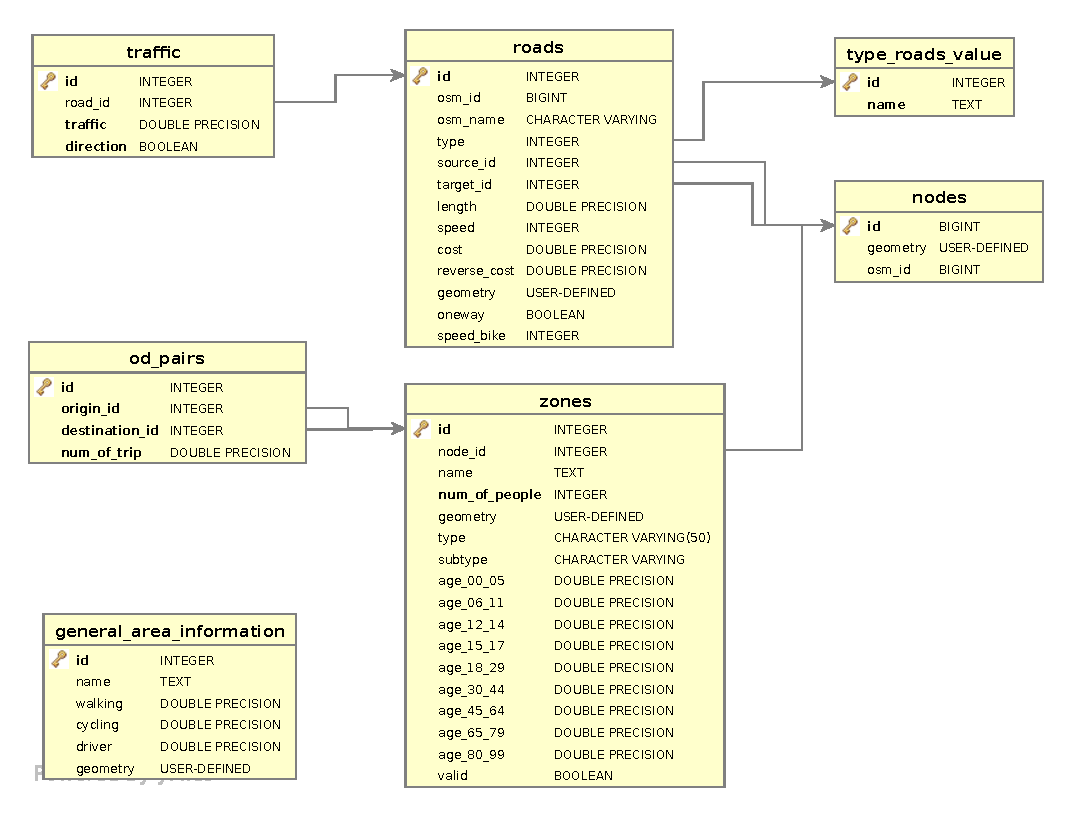
\includegraphics[width=15cm]{img/db.eps}
\caption{DB model}
\end{figure}

More details about DB you can find in project documentation on GitHub.

s03-practice.tex

\chapter{Web content}
% Application - Prototypes
%%%%%%%%%%%%%%%%%%%%%%%%%%%%%%%%%%%%%%%%%%%%%

% FR
% Avant d'entamer le développement de l'application, il est nécessaire de faire un état du besoin et des attentes. Ainsi, en structurant notre interface il sera plus facile de procéder à son développement graphique, d'anticiper les classes et fonctions nécessaires aux traitements. Dans un premier temps, nous allons structurer nos interfaces afin d'être au plus proche des attentes utilisateurs, puis nous détaillerons les outils à notre disposition et comment ils fonctionnent, et enfin nous procèderons au dévelopement de l'application cliente.

% EN
Before starting the development of the application, it is necessary to make a statement of needs and expectations. Thus, by structuring our interface will make it easier to conduct its graphic development, anticipate the classes and functions necessary for treatment. Initially, we will structure our interfaces in order to be closer to the users expectations, then we will detail the tools available and how they work, and then we will proceed to the developement of the client application.

% FR
%\section{Prototypes}

% EN
\section{Prototypes}

% FR
%Dans ce paragraphe nous allons détailler chacune des interfaces qui seront implémentées dans l'application. L'application sera construite sous deux angles différents :
% \begin{description}
%   \item[La partie cartographique :] \hfill \\ contenant une carte de base et dont les outils se superposent à cette dernière
%   \item[La partie site web :] \hfill \\ contenant des outils indépendants de la carte
% \end{description}

% EN
In this section we will detail each of the interfaces that will be implemented in the application. The application will be built in two different ways:
\begin{description}
  \item[Map content :] \hfill \\ containing a basemap and whose tools are over the map
  \item[Website content :] \hfill \\ containing independent map tools
\end{description}

% FR
%\subsection{Partie cartographique}

% EN
\subsection{Map content}

Lorem ipsum dolor sit amet, consectetur adipiscing elit. Morbi luctus varius consequat. Donec id nisl vel nisi pretium dictum sagittis quis massa. Suspendisse scelerisque ex velit, et aliquam ante aliquam id. Ut quis augue sagittis, lacinia eros condimentum, dignissim velit. Curabitur enim sapien, vehicula volutpat dui ut, finibus suscipit eros. 

% BASEMAP
% ----------------------------------------------
Lorem ipsum dolor sit amet, consectetur adipiscing elit. Morbi luctus varius consequat. Donec id nisl vel nisi pretium dictum sagittis quis massa. Suspendisse scelerisque ex velit, et aliquam ante aliquam id. Ut quis augue sagittis, lacinia eros condimentum, dignissim velit. Curabitur enim sapien, vehicula volutpat dui ut, finibus suscipit eros. 

\begin{figure}[ht]
    \centering
    \begin{subfigure}[b]{0.6\textwidth}
        \includegraphics[width=\textwidth]
          {img/c02-application/png/web-basemap.png}
        \caption{Web}
    \end{subfigure}
    ~
    \begin{subfigure}[b]{0.2\textwidth}
        \includegraphics[width=\textwidth]
          {img/c02-application/png/mobile-basemap.png}
        \caption{Mobile}
    \end{subfigure}
    \caption{Application: Basemap}
\end{figure}

% TOC
% ----------------------------------------------
Lorem ipsum dolor sit amet, consectetur adipiscing elit. Morbi luctus varius consequat. Donec id nisl vel nisi pretium dictum sagittis quis massa. Suspendisse scelerisque ex velit, et aliquam ante aliquam id. Ut quis augue sagittis, lacinia eros condimentum, dignissim velit. Curabitur enim sapien, vehicula volutpat dui ut, finibus suscipit eros. 

\begin{figure}[ht]
    \centering
    \begin{subfigure}[b]{0.6\textwidth}
        \includegraphics[width=\textwidth]
          {img/c02-application/png/web-basemap-toc.png}
        \caption{Web}
    \end{subfigure}
    ~
    \begin{subfigure}[b]{0.2\textwidth}
        \includegraphics[width=\textwidth]
          {img/c02-application/png/mobile-basemap-toc.png}
        \caption{Mobile}
    \end{subfigure}
    \caption{Application: Table Of Content}
\end{figure}

% SEARCH POINTER
% ----------------------------------------------
Lorem ipsum dolor sit amet, consectetur adipiscing elit. Morbi luctus varius consequat. Donec id nisl vel nisi pretium dictum sagittis quis massa. Suspendisse scelerisque ex velit, et aliquam ante aliquam id. Ut quis augue sagittis, lacinia eros condimentum, dignissim velit. Curabitur enim sapien, vehicula volutpat dui ut, finibus suscipit eros. 

\begin{figure}[ht]
    \centering
    \begin{subfigure}[b]{0.6\textwidth}
        \includegraphics[width=\textwidth]
          {img/c02-application/png/web-basemap-search.png}
        \caption{Web}
    \end{subfigure}
    ~
    \begin{subfigure}[b]{0.2\textwidth}
        \includegraphics[width=\textwidth]
          {img/c02-application/png/mobile-basemap-search.png}
        \caption{Mobile}
    \end{subfigure}
    \caption{Application: SearchPointer}
\end{figure}

% FOCUS
% ----------------------------------------------
Lorem ipsum dolor sit amet, consectetur adipiscing elit. Morbi luctus varius consequat. Donec id nisl vel nisi pretium dictum sagittis quis massa. Suspendisse scelerisque ex velit, et aliquam ante aliquam id. Ut quis augue sagittis, lacinia eros condimentum, dignissim velit. Curabitur enim sapien, vehicula volutpat dui ut, finibus suscipit eros. 

\begin{figure}[ht]
    \centering
    \begin{subfigure}[b]{0.6\textwidth}
        \includegraphics[width=\textwidth]
          {img/c02-application/png/web-basemap-focus.png}
        \caption{Web}
    \end{subfigure}
    ~
    \begin{subfigure}[b]{0.2\textwidth}
        \includegraphics[width=\textwidth]
          {img/c02-application/png/mobile-basemap-focus.png}
        \caption{Mobile}
    \end{subfigure}
    \caption{Application: Focus}
\end{figure}

% CONTACT
% ----------------------------------------------
Lorem ipsum dolor sit amet, consectetur adipiscing elit. Morbi luctus varius consequat. Donec id nisl vel nisi pretium dictum sagittis quis massa. Suspendisse scelerisque ex velit, et aliquam ante aliquam id. Ut quis augue sagittis, lacinia eros condimentum, dignissim velit. Curabitur enim sapien, vehicula volutpat dui ut, finibus suscipit eros. 

\begin{figure}[ht]
    \centering
    \begin{subfigure}[b]{0.6\textwidth}
        \includegraphics[width=\textwidth]
          {img/c02-application/png/web-basemap-contact.png}
        \caption{Web}
    \end{subfigure}
    ~
    \begin{subfigure}[b]{0.2\textwidth}
        \includegraphics[width=\textwidth]
          {img/c02-application/png/mobile-basemap-contact.png}
        \caption{Mobile}
    \end{subfigure}
    \caption{Application: Contact}
\end{figure}

% FR
%\subsection{Partie site web}

% EN
\subsection{Website content}

% STATS
% ----------------------------------------------
Lorem ipsum dolor sit amet, consectetur adipiscing elit. Morbi luctus varius consequat. Donec id nisl vel nisi pretium dictum sagittis quis massa. Suspendisse scelerisque ex velit, et aliquam ante aliquam id. Ut quis augue sagittis, lacinia eros condimentum, dignissim velit. Curabitur enim sapien, vehicula volutpat dui ut, finibus suscipit eros. 

\begin{figure}[ht]
    \centering
    \begin{subfigure}[b]{0.6\textwidth}
        \includegraphics[width=\textwidth]
          {img/c02-application/png/web-website-stats.png}
        \caption{Web}
    \end{subfigure}
    ~
    \begin{subfigure}[b]{0.2\textwidth}
        \includegraphics[width=\textwidth]
          {img/c02-application/png/mobile-website-stats.png}
        \caption{Mobile}
    \end{subfigure}
    \caption{Application: Statistics}
\end{figure}

% TIMETABLES
% ----------------------------------------------
Lorem ipsum dolor sit amet, consectetur adipiscing elit. Morbi luctus varius consequat. Donec id nisl vel nisi pretium dictum sagittis quis massa. Suspendisse scelerisque ex velit, et aliquam ante aliquam id. Ut quis augue sagittis, lacinia eros condimentum, dignissim velit. Curabitur enim sapien, vehicula volutpat dui ut, finibus suscipit eros. 

\begin{figure}[ht]
    \centering
    \begin{subfigure}[b]{0.6\textwidth}
        \includegraphics[width=\textwidth]
          {img/c02-application/png/web-website-timetables.png}
        \caption{Web}
    \end{subfigure}
    ~
    \begin{subfigure}[b]{0.2\textwidth}
        \includegraphics[width=\textwidth]
          {img/c02-application/png/mobile-website-timetables.png}
        \caption{Mobile}
    \end{subfigure}
    \caption{Application: Timetables}
\end{figure}

% Application - Code
%%%%%%%%%%%%%%%%%%%%%%%%%%%%%%%%%%%%%%%%%%%%%

\section{Development}

Lorem ipsum dolor sit amet, consectetur adipiscing elit. Sed tempus faucibus nisi maximus commodo. Suspendisse potenti. Duis viverra scelerisque sem, ac convallis nibh tristique commodo. Donec quis leo id ligula eleifend efficitur sed vel est. Mauris ac pharetra erat. Fusce sit amet ligula elementum, aliquet sem in, aliquam tortor. Sed dapibus leo vel facilisis commodo. Sed porttitor nisl sem, eu ultricies dui fermentum a. Cras sed dictum leo, ut posuere turpis. Pellentesque interdum nisl odio, ut accumsan mauris fermentum a. Aliquam accumsan sagittis magna, a sodales magna sagittis quis. Nulla rutrum nisl libero, sit amet egestas arcu consectetur vitae. Aliquam fringilla rutrum auctor. Nullam tempor placerat massa, quis gravida nisi dignissim vitae. 
s03-practice.tex

\chapter{Merge}
s01-data.tex
\input{./chapter/c03-merge/s02-app_model.tex}

\chapter*{Conclusion}
\addcontentsline{toc}{chapter}{Introduction}
% CONCLUSION
%%%%%%%%%%%%%%%%%%%%%%%%%%%%%%%%%%%%%%%%%%%%%

% FR
% L'information représente un actif important lié aux systèmes d'information géographique, dans le contexte actuel, la concurrence effrénée à laquelle se livrent les entreprises entraîne la multiplication des SIG comme atout majeur lors des décisions stratégiques.

% EN
Information is an important asset related to geographic information systems, in the current context, the unbridled competition that companies indulge causes the proliferation of GIS as a major asset in strategic decisions.

We done web application about transport information for Finland data source. Demo area is for city Hyvinkää in south Finland. Application is focused on bike traffic visualization with some additional function as finding shortest path.

Our solution can split to 2 part frontend and backend. Frontend is written in JavaScript using Leaflet. Backend is written in python using Python, Flask.

% FR


% EN










% BIBLIOGRAPHIE
%--------------------------------------
% TODO: Bibliography
\begin{thebibliography}{ABC}

  \bibitem[REF] {Leaflet} 
    \url{http://leafletjs.com/}\\
    \emph{Leaflet website}. 
    2015 Vladimir Agafonkin. Maps - OpenStreetMap contributors.

  \bibitem[REF] {Leaflet-extension : Sidebar} 
    \url{https://github.com/Turbo87/leaflet-sidebar}\\
    \emph{Leaflet extension Sidebar}. 
    leaflet-sidebar is free software, and may be redistributed under the MIT license.

  \bibitem[REF] {Leaflet-extension : EasyButton} 
    \url{https://github.com/CliffCloud/Leaflet.EasyButton}\\
    \emph{Leaflet extension EasyButton}. 
    Leaflet-EasyButton maintained by CliffCloud

  \bibitem[REF] {Bootstrap} 
    \url{http://getbootstrap.com/}\\
    \emph{Bootstrap CSS Framework website}.
    Code licensed under MIT, documentation under CC BY 3.0. 

  \bibitem[REF] {Bootstrap-extension Select} 
    \url{http://silviomoreto.github.io/bootstrap-select/}\\
    \emph{Bootstrap extension Select}.
    Bootstrap-select maintained by caseyjhol 

  \bibitem[REF] {Cordova} 
    \url{https://cordova.apache.org/}\\
    \emph{Cordova website}.
    Copyright 2012, 2013, 2015 The Apache Software Foundation, Licensed under the Apache License, Version 2.0 

  \bibitem[REF] {JsDoc} 
    \url{https://github.com/jsdoc3/jsdoc}\\
    \emph{JsDoc3 : Generate Javascript documentation}.
    JSDoc 3 is free software, licensed under the Apache License, Version 2.0. 
    
  \bibitem[REF] {postgis} 
    \url{http://postgis.net/docs/manual-2.0/}\\
    \emph{PostGIS 2.0 Manual}.
    This work is licensed under a Creative Commons Attribution-Share Alike 3.0 License 
    
  \bibitem[REF] {iGraph} 
    \url{http://igraph.org/python/doc/igraph-module.html}\\
    \emph{python-igraph manual}.
    
  \bibitem[REF] {Flask} 
    \url{http://flask.pocoo.org/docs/0.10/}\\
    \emph{Flask’s documentation}.


\end{thebibliography}

% ANNEXES
%--------------------------------------
\appendix

\newpage

%%%%%%%%%%%%%%%%%%%%%%%%%%%%%%%%%%%%%%%%%%%%%

\setlength{\parskip}{0em}
\listoffigures
\listoftables

% GLOSSAIRE
%--------------------------------------

\addcontentsline{toc}{chapter}{Glossaire}
\printglossaries

\end{document}